\documentclass[a4paper,oneside,12 pt]{article}
\usepackage[french]{babel}
\usepackage[T1]{fontenc}
\usepackage{verbatim}
\usepackage[utf8]{inputenc}
\usepackage{multirow}
\usepackage{graphicx}

\title{Autour de Metaciv}

\date{}
\begin{document}

\maketitle

\newpage
\section{Méta-Modèle}

Inspiré par le modèle des cadrans, la plateforme Metaciv est fondé sur le  méta-modèle suivant.
\begin{figure}[!h]
\begin{center}
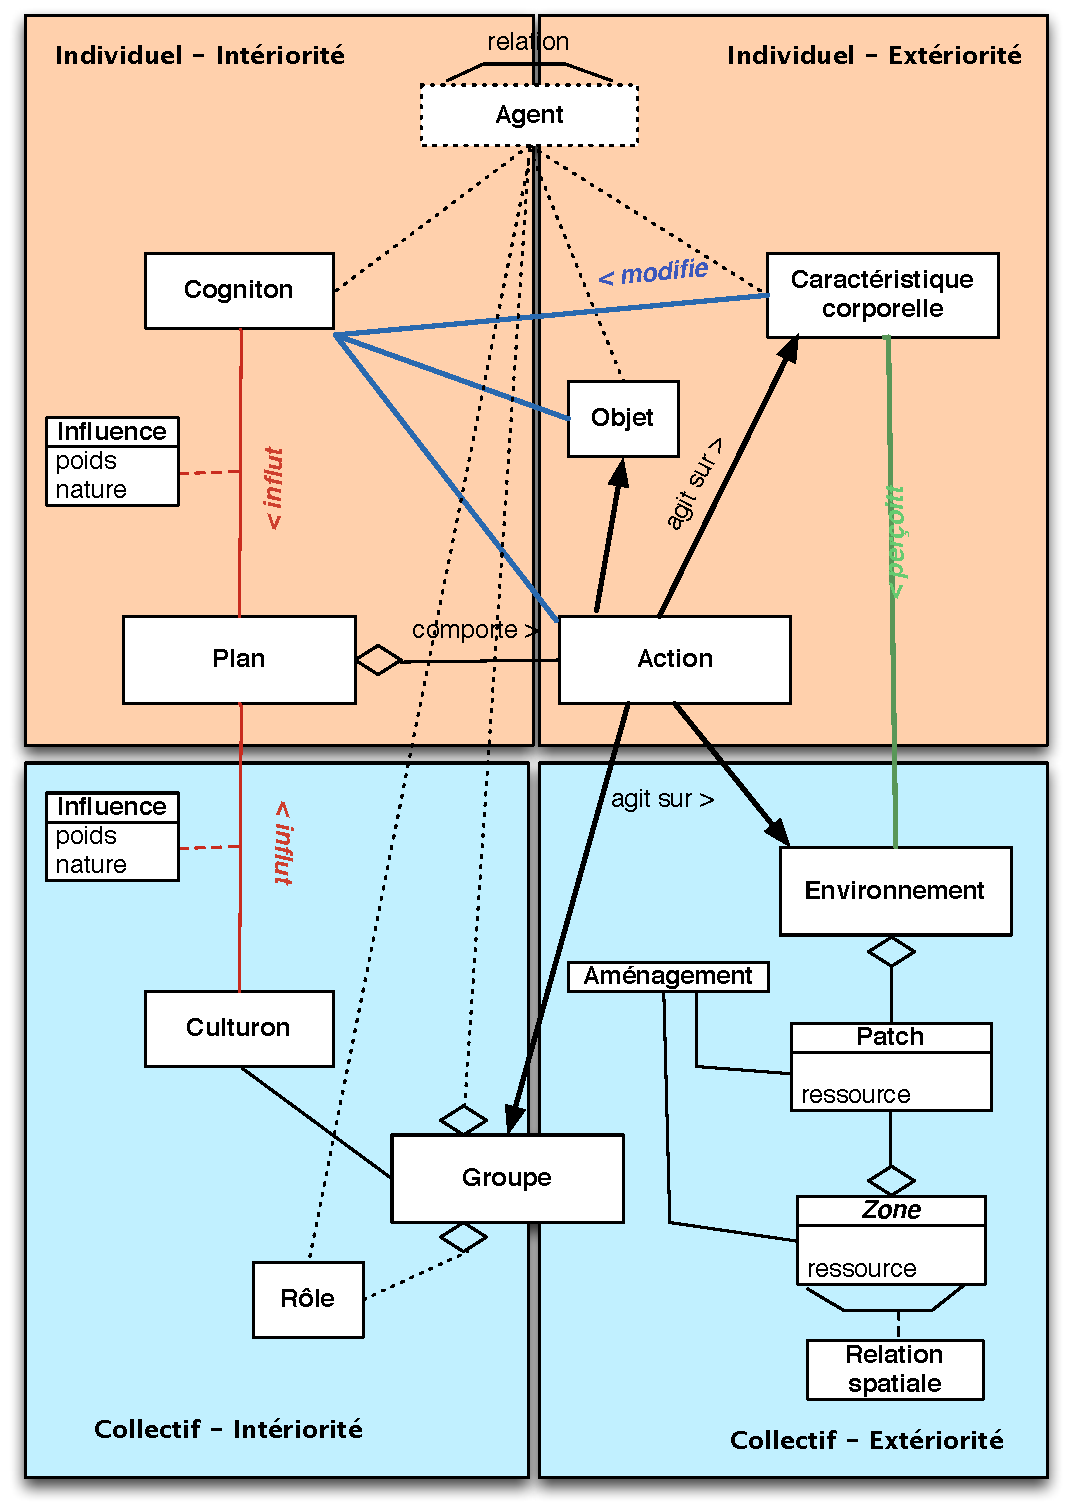
\includegraphics[scale=0.6]{modele.pdf}
\caption[Modele]{MétaModèle \\}
\label{ex1}
\end{center}
\end{figure} 
\section{Agent}
Les agents sont vus sous l'angle \textit{intériorité }comme dotés d'un esprit (ensemble de cognitons) qui leur permet d'établir des plans (ensemble d'actions) ;  vus sous l'angle \textit{extériorité} ils sont dotés d'un ensemble de caractéristiques (corps) et peuvent manipuler des objets. Ils évoluent dans un environnement collectif agrégat de \textit{patches}.
Les cognitions vont influencer les plans, de manière pondérée (selon l'importance que le modélisateur leur accorde), de manière positive (renforcement) ou négative (affaiblissement).
L'environnement ainsi que les actions effectuées peuvent affecter les caractéristiques d'un agent et de ce fait influer sur ses cognitons.
De même les actions peuvent directement ou indirectement via les objets influer sur les cognitons.
\subsection{Cognition}
\subsubsection{Notion de cognitons}
// à relire et améliorer
	Dans le cadre du projet Metaciv, il est très tôt apparu qu'il était nécessaire de gérer des agents disposant d'une capacité de réflexion relativement développée. 
	
	En effet, ceux-ci sont amenés à devoir opérer des choix dans un large panel d'actions.
	Dans cette optique, l'idée retenue consiste à pondérer les différentes actions possibles pour les agents, et  ce afin de les faire choisir en fonction de ces poids. 
	Les poids des actions sont déterminés par différents facteurs : ce que voient, pensent, croient les agents… L'ensemble de ces facteurs est regroupé sous le terme de « cogniton » dans ce projet, en reprenant le néologisme proposé par J. Ferber. Le cogniton est donc une « unité de pensée » qui influe sur les choix de l'agent. 	
	
	Les cognitons peuvent se cumuler, et ne sont donc pas des « états » mentaux. En fait, c'est la somme des cognitons qui représente réellement l'état mental de l'agent.
	
\subsubsection{Catégorisation des cognitons}

	Pour mieux structurer l'organisation des cognitons, ceux-ci sont catégorisés en cinq types :\textit{ Skills, Traits, Beliefs, Percepts, Mèmes}. Cette distinction permet de séparer des comportements différents entre ces cognitons, et de les traiter au mieux par la suite.
\begin{itemize}


\item 	Les\textit{ Skills} (signifiant compétences en anglais) représentent les compétences, savoir-faire et connaissances techniques ou scientifiques des agents. Comme exemples de ce type de cognitons, on peut proposer : Agriculture, Navigation, Fabrication d'outils… La plupart des skills ont la particularité d'être transmissibles d'un agent à l'autre, d'être permanents (ils ne disparaissent pas une fois acquis) et d'être des prérequis indispensables à certaines actions. 
	
	Par exemple, même si d'autres cognitons l'influencent, un agent ne peut pas fabriquer un outil si il ne dispose pas de Fabrication d'outils. Enfin, les skills sont héréditaires. Ici, on parle de l'hérédité au sens de la transmission entre les générations, ce qui représente de manière simple l'apprentissage et la transmission des connaissances.

\item 	Les \textit{Traits} représentent les spécificités individuelles de l'agent, ses traits de caractères, ses façons d'être. Des exemples possibles de ce type de cognitons sont : Ouvert, Renfermé, Paresseux…
	
	Cette catégorie n'est pas la plus importante du point de vue de la simulation et du réalisme, mais est un outil simple pour faire varier le comportement des agents si l'on veut envisager des scénarii spécifiques (des civilisations très agressives, des agents peu travailleurs, etc…). Les traits ne sont pas transmissibles d'agents à agents, sauf de manière héréditaire occasionnellement, ce qui représente l'imitation et l'éducation.

\item 	Les \textit{Beliefs} (Croyances en anglais) représentent ce que l'agent sait ou croit savoir de son environnement et de lui même. Cette catégorie est vaste, et peut regrouper des cognitons aussi variés que : Je porte une pioche, Nous sommes en guerre avec la civilisation 3, Je possède un champ. Ces cognitons ne sont généralement pas transmissibles entre agents, et ne sont pas héréditaires.

\item 	Les \textit{Percepts} représentent ce que l'agent voit, entend ou ressent (physiquement) au moment considéré. Des exemples de percepts sont : J'ai faim, Un ennemi est proche, Je suis près de l'eau. Ce type de cogniton est constamment retiré ou ajouté, contrairement aux autres types qui sont plus stables. Les percepts ne sont pas transmissibles, ils sont propres à l'agent considéré.

\item 	Les \textit{Mèmes}, d'après le terme inventé par R.Dawkins [2]. Son sens varie suivant les sources. Dans notre cas, nous définissons un mème comme étant une croyance ou un comportement culturel transmissible. Ainsi, les mèmes pourraient être : Je crois que l'argent est une fin en soi, je crois en l'existence d'un dieu, je crois que la démocratie est une bonne chose. Typiquement, les opinions religieuses et politiques sont des mèmes. Par définition, les mèmes sont transmissibles, et ils sont potentiellement héréditaires.
	
Les cognitons ont un poids qui par défaut est 1 (et qui peut être modifié par une action ou  par l'effet d'un objet ou par les culturons)
\end{itemize}
\subsection{Objets}
Les objets peuvent être créés selon les besoins par les agents (à partir d'un concept d'objet précédemment définis : parmi ces concepts on distingue les objets simples et composites). Les objets feront ensuite partie de l'inventaire d'un agent. Les objets peuvent avoir un effet sur des caractéristiques d'un agent ou sur des actions. 
\subsection{Plan et actions}
Les plans sont des ensembles d'actions et sont liés à des cognitons qui les influencent.
\subsection{Groupe et rôle}
à compléter ..
\section{Le  logiciel}
\subsection{Préambule}
MetaCiv, dans sa forme actuelle est un \textit{framework} permettant de mettre en place des modèles de simulation de sociétés/civilisations. Il repose sur MadKit (qui offre un mécanisme de gestion multi-agents) et TurtleKit (qui fournit en particulier l’interface et la gestion « physique » des agents).

Les principaux outils fournis par MetaCiv sont :
\begin{itemize}
\item Système « cognitif » pour les agents
\item Gestion de l’environnement à base de ressources (Cf. phéromones de Turtle Kit)
\item Outils de visualisation
\item Outils d’édition graphique
\end{itemize}
\subsection{Installation}

Il faut disposer du langage de programmation Java (version au moins 1.7) et récupérer le dossier Metaciv qui contient le dossier \textit{Launcher} ainsi que divers modèles exemples dans le Dropbox.

Ouvrir de dossier \textit{Launcher}, double clic sur le module \textit{Metaciv+numversion.jar}


Une fenêtre s'ouvre, il faut alors rechercher et ouvrir le fichier de paramètres initiaux  \texttt{parametres.metaciv} dans le modèle choisi. (Chaque modèle a un fichier de paramétrage)



\begin{figure}[hbtp]
\begin{center}
 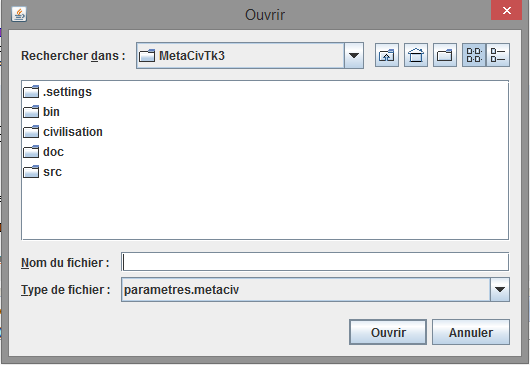
\includegraphics [scale=0.4] {ecran1.png}
\end{center}
 \caption{Le choix du fichier de paramétrage initial}
\end{figure}

%\newpage

Deux fenêtres, constituant l'environnement de fonctionnement de Metaciv  s'ouvrent alors : 

l'une \textit{worldviewer} propose un fond cartographique par défaut (environnement d'évolution)

\begin{figure}[hbtp]
\begin{center}
 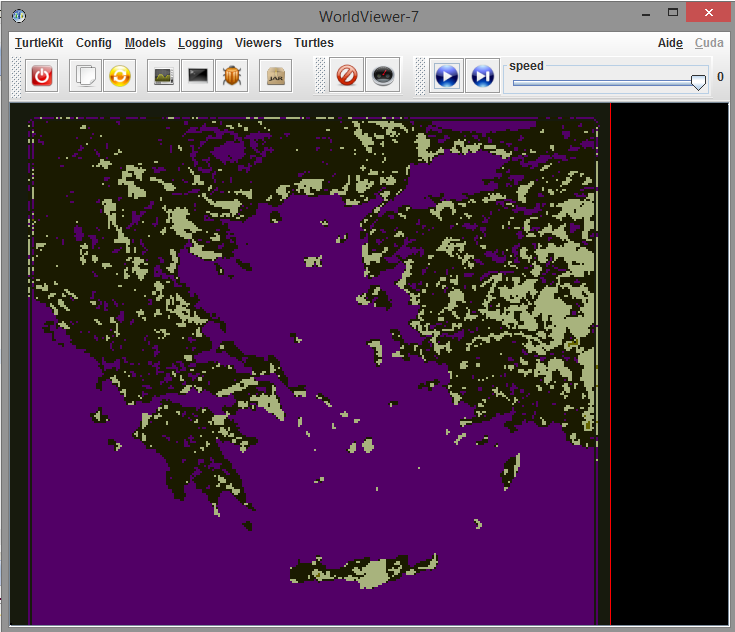
\includegraphics [scale=0.5] {worldviewer.png}
\end{center}
 \caption{La vision de l'environnement de simulation}
\end{figure}
\newpage

l'autre \textit{wiewertab} 

\begin{figure}[hbtp]
\begin{center}
 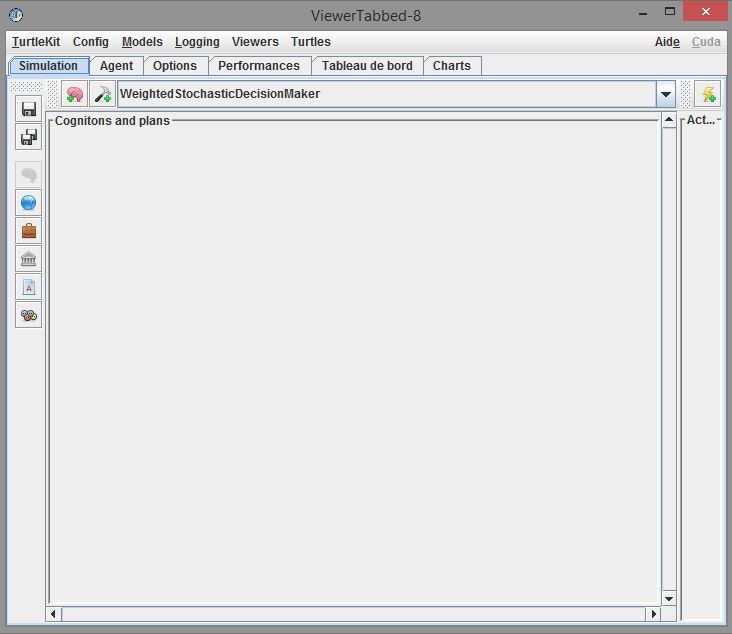
\includegraphics [scale=0.5] {viewertabbed.png}
\end{center}
 \caption{La vision de la fenêtre entrée / sortie pour le modélisateur}
\end{figure}


Les onglets de la ligne supérieure sont réservés aux experts \textit{turtlekit}.
\newpage



La ligne suivante propose des onglets permettant d'accéder à différents détails 
\begin{figure}[hbtp]
\begin{center}
 
\includegraphics [scale=0.5] {Onglets.pdf}
\end{center}
 \caption{Les onglets accessibles }
\end{figure}


\begin{itemize}
\item L'onglet\textit{ Simulation} dispose d'une palette d'icônes permettant la création du modèle et permet la modification de la simulation.
Cet onglet contient deux barres d’outils, la barre du haut varie en fonction du domaine de la simulation que l’on souhaite éditer, celle de gauche permet de naviguer grâce à des icônes parmi les différents domaines éditables.
\begin{itemize}
\item \textbf{Population ou société}
par défaut il s'agit d'un ensemble d'agents homogènes ( 1 ou n) situé initialement sur un patch ou zone choisie sur l'environnement (clic droit). On peut donc au départ créer plusieurs populations mais constituée d'agents initialement identiques.
\item \textbf{Caractéristiques}
pour chacune définir son nom et sa valeur initiale (exemple  vie 100)
\item \textbf{Groupes}
permet de structurer les populations initiales (à compléter )
\end{itemize}

\begin{figure}[hbtp]
\begin{center}
 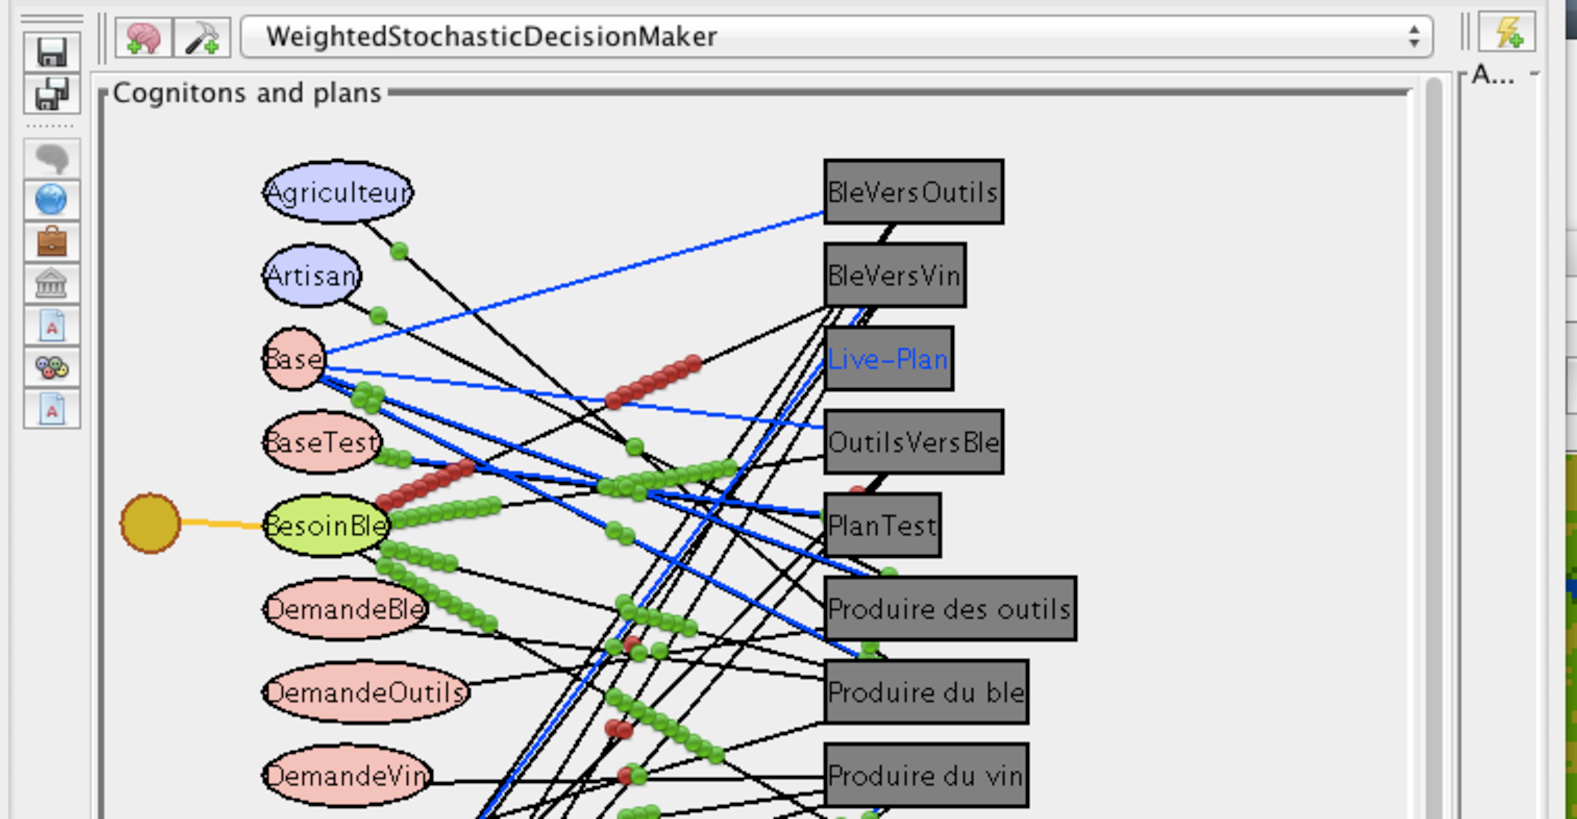
\includegraphics [scale=0.5] {Simul.pdf}
\end{center}
 \caption{Les icônes de l'onglet Simulation }
\end{figure}


\item L'onglet \textit{Agents} : Affiche des informations sur les agents, permet de sélectionner l’agent à observer en navigant par ID.
%\item Communautés : Onglet obsolète (qui sera amené à être amélioré).
\item L'onglet \textit{Options} : permet de positionner différentes options (en particulier d’affichage). 

\item  L'onglet \textit{Performances} : présente différentes informations sur la consommation mémoire.
\item L'onglet \textit{Tableau de bord} : offre quelques outils de visualisation, par exemple le ratio des cognitons (sous forme de camembert)
\item L'onglet \textit{Charter} : présente des graphiques de synthèse et le poids des plans 

\end{itemize}


	

	
	

	
	

	







%L'onglet Agent
%lorsque la simulation s'exécute on peut observer divers détails
%les groupes
%l'inventaire (les objets)
%relation entre agents (à rajouter)
%plans 
%cognitons
%L'onglet Options
%options de visualisation
%action sur la visualisation des agents 
%changement d'une carte (couleur du patch) en fn d'une ressource d'un patch
%choix d'un groupe ou d'un rôle
%L'onglet PERFORMANCES 
%L'onglet tableau de bord 



Le modélisateur doit donc créer toutes entités nécessaires à son modèle (ce qui nécessite une phase de réflexion et la connaissance d'un méta-langage afin d'invoquer des codes préexistants).

Lorsque l'univers est créé, revenir sur la fenêtre \textit{worldviewer} et cliquer sur l'icône Play (on peut régler la vitesse d'exécution) et éventuellement passer en mode pas à pas.
Il est possible d'effectuer des Zooms sur l'environnement  avec la souris 
A noter la présence du bouton fin qui clôt la simulation (impératif).

Si l'on souhaite avoir des détails relatifs aux agents, on peut arrêter la simulation puis 
Clic gauche sélection d'un ou de plusieurs agents
Clic droit pour l'observation. Cela ouvre une nouvelle fenêtre avec plusieurs onglets
\begin{figure}[hbtp]
\begin{center}
 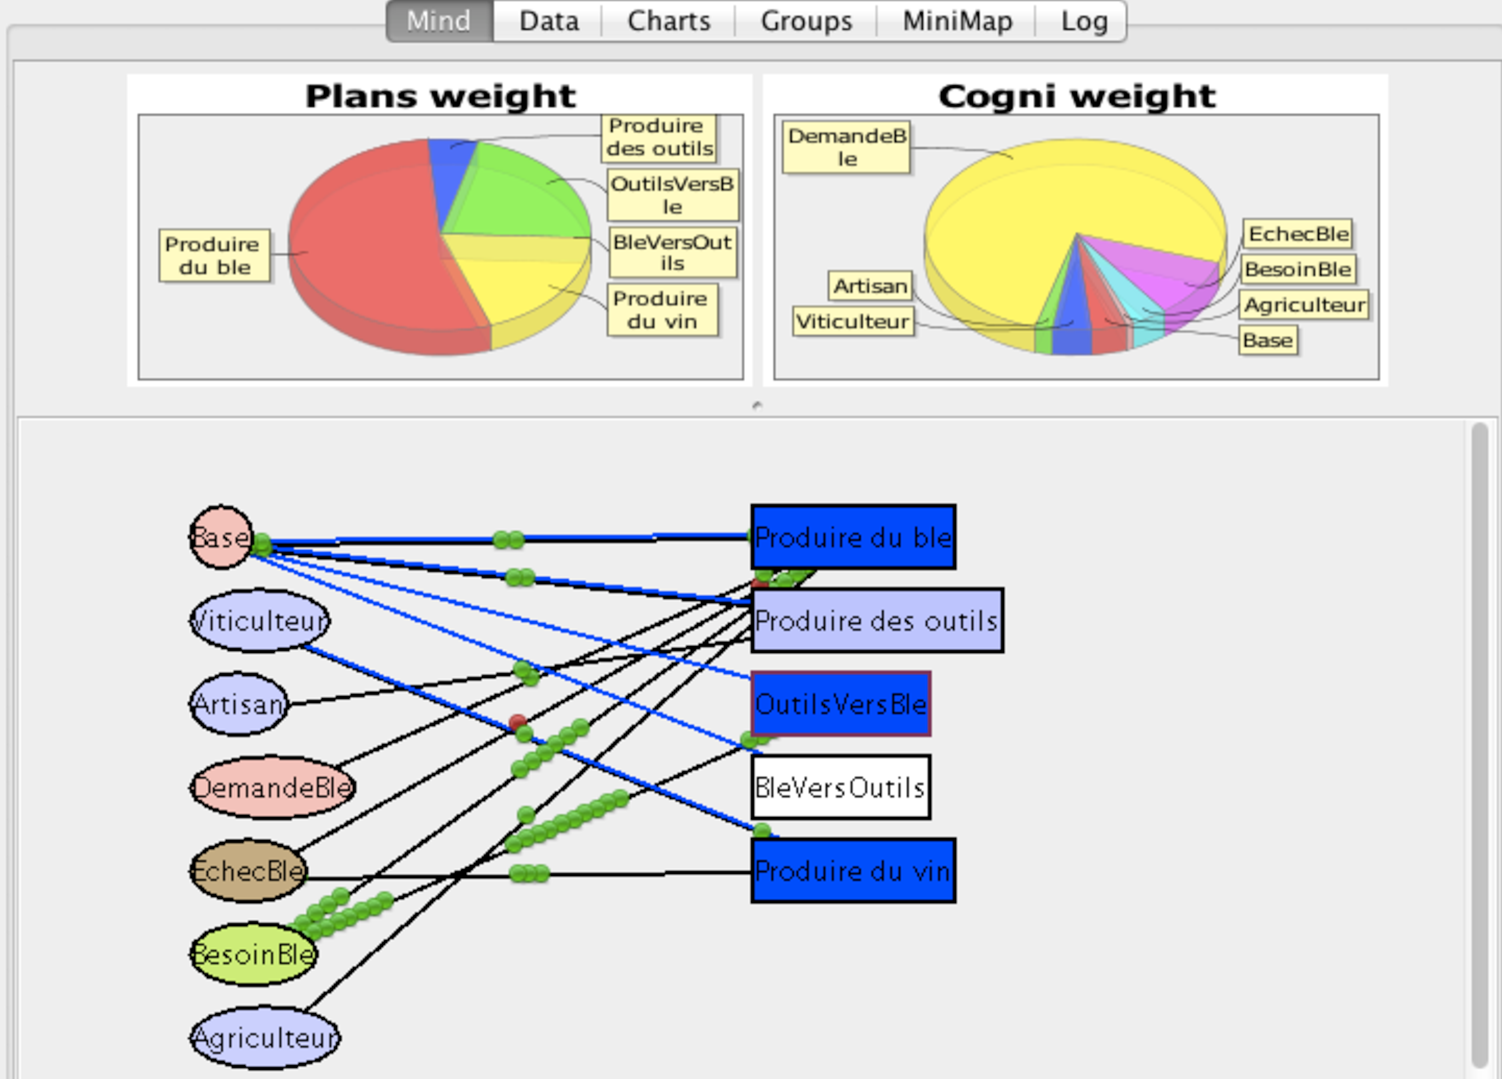
\includegraphics [scale=0.5] {Observe.pdf}
\end{center}
 \caption{Les onglets liés à l'observation }
\end{figure}
\begin{itemize}
\item Onglet \textit{ Mind}
affiche l'esprit (plan et cogniton poids ds le haut et  lien coginiton ds le bas)
\item Onglet \textit{Data}
affiche les caractéristiques de l'agent (ou des agents)
\item Onglet\textit{ Charts}
attributs
\item Onglet \textit{Groups}
role et groupe
\item Onglet\textit{ Minimap}
zoom 
\item Onglet \textit{Log}
Historique de l'exécution des plans (séquentiel .. mais attribution aléatoire du poids)
\end{itemize}


\end{document}